\documentclass[twoside]{article}
\usepackage[a4paper]{geometry}
\geometry{verbose,tmargin=2.5cm,bmargin=2cm,lmargin=2cm,rmargin=2cm}
\usepackage{fancyhdr}
\pagestyle{fancy}

% nastavení pisma a~češtiny
\usepackage{lmodern}
\usepackage[T1]{fontenc}
\usepackage[utf8]{inputenc}
\usepackage[czech]{babel}

% odkazy
\usepackage{url}

\usepackage{float}
% vícesloupcové tabulky
\usepackage{multirow}
\usepackage{listings}
\usepackage{xcolor}
\usepackage{amssymb}
\usepackage{gensymb}
\usepackage{bbold}
\usepackage{amsmath}
\usepackage{siunitx}
\usepackage{mathtools}
\usepackage{commath}

% vnořené popisky obrázků
\usepackage{subcaption}

% automatická konverze EPS 
\usepackage{graphicx} 
\usepackage{epstopdf}
\epstopdfsetup{update}

\graphicspath{{./images}}

% odkazy a~záložky
\usepackage[unicode=true, bookmarks=true,bookmarksnumbered=true,
bookmarksopen=false, breaklinks=false,pdfborder={0 0 0},
pdfpagemode=UseNone,backref=false,colorlinks=true] {hyperref}


% Poznámky při překladu
\usepackage{xkeyval}	% Inline todonotes
\usepackage[textsize = footnotesize]{todonotes}
\presetkeys{todonotes}{inline}{}

%https://tex.stackexchange.com/questions/2783/bold-calligraphic-typeface
\DeclareMathAlphabet\mathbfcal{OMS}{cmsy}{b}{n}

% enumerate zacina s pismenem
\renewcommand{\theenumi}{\alph{enumi}}

% smaz aktualni page layout
\fancyhf{}
% zahlavi
\usepackage{titling}
\fancyhf[HC]{\thetitle}
\fancyhf[HLE,HRO]{\theauthor}
\fancyhf[HRE,HLO]{\today}
 %zapati
\fancyhf[FLE,FRO]{\thepage}

% údaje o autorovi
\title{OTE Domácí úkol 8 - Synchronní detekce}
\author{Vojtěch Michal}
\date{\today}

%customize code listing
\definecolor{codegreen}{rgb}{0,0.6,0}
\definecolor{codegray}{rgb}{0.5,0.5,0.5}
\definecolor{codepurple}{rgb}{0.58,0,0.82}
\definecolor{backcolour}{rgb}{0.95,0.95,0.92}

\lstdefinestyle{mystyle}{
    backgroundcolor=\color{backcolour},   
    commentstyle=\color{codegreen},
    keywordstyle=\color{magenta},
    numberstyle=\tiny\color{codegray},
    stringstyle=\color{codepurple},
    basicstyle=\ttfamily\footnotesize,
    breakatwhitespace=false,         
    breaklines=true,                 
    captionpos=b,                    
    keepspaces=true,                 
    numbers=left,                    
    numbersep=5pt,                  
    showspaces=false,                
    showstringspaces=false,
    showtabs=false,                  
    tabsize=2
}

\lstset{style=mystyle}

\begin{document}

\maketitle

Simulační schéma synchronního detektoru je na obrázku \ref{schema}.
Paralelní zapojení R2 a C1 simuluje měřenou impedanci,
která je buzená ze zdroje V1 a intvertujícím zesilovačem A1
převáděna na napětí. V pravé části obvodu kolem A2 je zesilovač s přepínatelným
zesílením  $\pm 1$ s uzemněným spínačem S1. Manuální přepínač S2
umožňuje výběr řídicího signálu pro spínač S1 mezi žádným fázovým posunem z V1
(pro měření reálné složky impedance) a fázovým posunem 90° z V2 (pro imaginární složku impedance).
Budicí napětí generované zdrojem V1 je v textu označneo jako $U_1$, výstupní napětí na uzlu 5
je $U_2$.

\begin{figure}[h]
    \centering
    \includegraphics[width=\textwidth]{schema.png}
    \caption{Simulační schéma}
    \label{schema}
\end{figure}
\clearpage

\section{Ověření funkce obvodu}

Odpojením kapacity C1, nastavením R2 = \SI{1}{\mega\ohm} 
a použitím fázově neposunutého buzení
se celé zapojení zjednodušuje na dvoucestný usměrňovač, jehož převodní charakteristika
je vykeslena na obrázku \ref{dvoucest-usmernovac}. Na levé
svislé ose je velikost výstupního napětí $U_2$ obvodu,
na pravé svislé ose je odchylka skutečné převodní charakteristiky od
ideální $U_2 = \text{abs}\,(U_1)$. Je patrná chyba menší než \SI{1}{\milli\volt}
napříč celým rozsahem měření.

\begin{figure}[h]
    \centering
    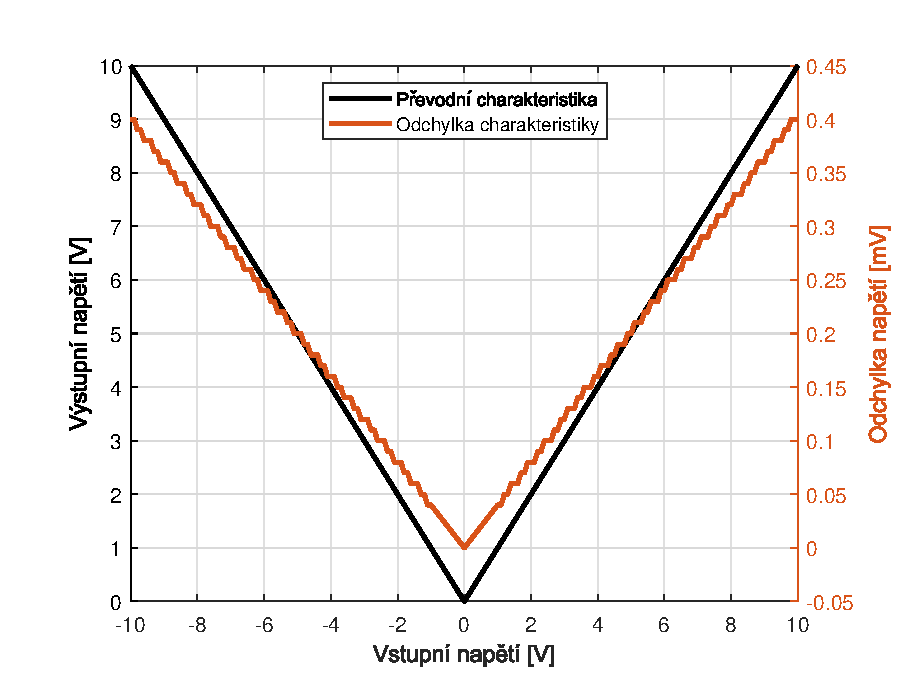
\includegraphics[width=\textwidth]{char-dvoucest-usmernovac.eps}
    \caption{Převodní charakteristika dvojcestného usměrňovače}
    \label{dvoucest-usmernovac}
\end{figure}

Posunutím buzení o 90° byla měřena imaginární složka impedance.
S odpojenou kapacitou C1 by měl být výstup obvodu nulový.
Změřené hodnoty jsou sepsány v tabulce \ref{odpojene-c-imag}.
Výstupní napětí je skutečně skoro nulové a jen
málo závislé na velikosti reálné složky měřené impedance.
\begin{table}[h]
    \centering
    \begin{tabular}{c|c}
        Odpor R2 [M$\Omega$] & $U_2$ [mV] \\ \hline
        1 & -8.3 \\ 
        2 & -3.1 \\ 
        3 & -2.8 \\ 
        4 & -1.4 \\ 
        5 & -1.1 \\ 
    \end{tabular}
    \caption{Imaginární složka napětí při odpojené kapacitě C1 v závislosti na nastaveném odporu R2}
    \label{odpojene-c-imag}
\end{table}
\clearpage

\section{Měření kapacity}

Podle zadání bylo nastaveno R1 = \SI{5}{\mega\ohm}, R3 = \SI{1}{\mega\ohm}
a byl použit
budicí signál o efektivní hodnotě \SI{5}{\volt} a frekvenci \SI{1}{\kilo\hertz}.
Pro měření imaginární složky impedance je spínač S1 je řízen signálem fázově posunutým o 90° vůči buzení.
Závislost výstupního napětí na nastavené kapacitě je zachycena v tabulce \ref{tab-c}.
Kapacity uvedené ve třetím sloupci byly vypočteny podle vzorce
\begin{equation}
    C =\frac{1.11 \text{Im}(U_2)}{2\pi f R_3 U_1} = \frac{1.11 \text{Im}(U_2)}{2\pi \cdot 10^3 \cdot 10^6\cdot 5}.
\end{equation}
Data jsou vykreslena na obrázku \ref{mereni-c}. Imaginární složka impedance je vypočtená
s přesností lepší než \SI{0.5}{\pico\farad} v celém rozsahu.

\begin{table}[h]
    \centering
    \begin{tabular}{c|c|c}
        nastavená kapacita C1 [pF] & střední hodnota výstupního napětí [V] & spočtená kapacita [pF] \\\hline
        10 & 0.2800 &   9.8931 \\
        20 & 0.5770 &  20.3868 \\
        30 & 0.8500 &  30.0325 \\
        40 & 1.1360 &  40.1376 \\
        50 & 1.4260 &  50.3840 \\
        60 & 1.7050 &  60.2417 \\
        70 & 1.9880 &  70.2408 \\
        80 & 2.2730 &  80.3105 \\
        90 & 2.5540 &  90.2389 \\
       100 & 2.8380 & 100.2733 \\
    \end{tabular}
    \caption{Měření kapacity synchronním detektorem}
    \label{tab-c}
\end{table}

\begin{figure}[h]
    \centering
    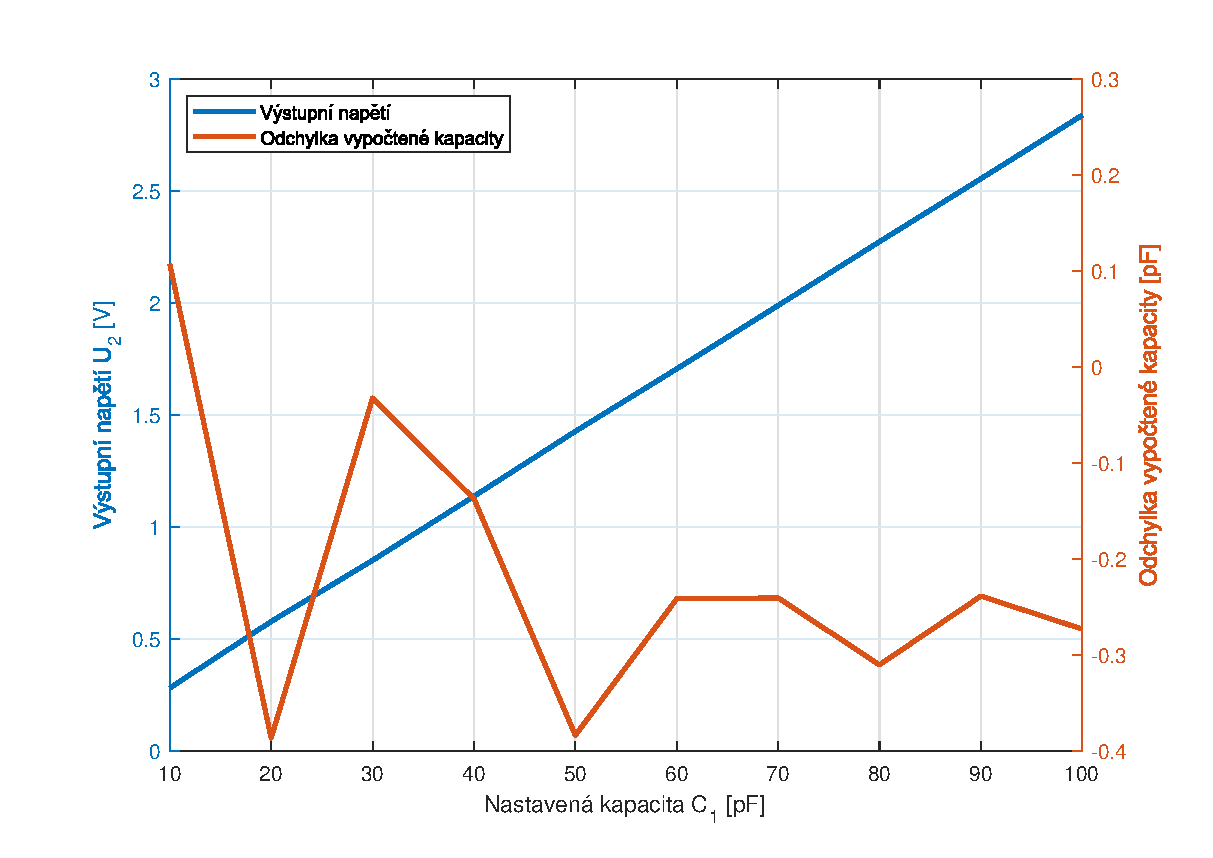
\includegraphics[width=\textwidth]{mereni-c.eps}
    \caption{Chyba měření kapacity synchronním detektorem}
    \label{mereni-c}
\end{figure}

\clearpage
\section{Měření odporu}

Podle zadání bylo nastaveno R3 = \SI{1}{\mega\ohm}, C1 = \SI{50}{\pico\farad}
a byl použit budicí signál o efektivní hodnotě \SI{5}{\volt} a frekvenci \SI{1}{\kilo\hertz}.
Spínač S1 je řízen ve fázi s budicím signálem pro měření reálné složky impedance.
Závislost výstupního napětí na ztrátovém odporu je zachycena v tabulce \ref{tab-r}.
Odpory uvedené ve třetím sloupci byly vypočteny podle vzorce
\begin{equation}
    R = \frac{U_1 R_3}{1.11 \text{Re}(U_2)} = \frac{5 \cdot 10^6}{1.11 \text{Re}(U_2)}.
\end{equation}
Data jsou vykreslena na obrázku \ref{mereni-r}. Reálná složka impedance je vypočtená
s přesností lepší než \SI{0.3}{\mega\ohm} v celém rozsahu.

\begin{table}[h]
    \centering
    \begin{tabular}{c|c|c}
        nastavený odpor R2 [M$\Omega$] & střední hodnota výstupního napětí [V] & spočtený odpor [M$\Omega$] \\\hline
        1 & 4.5820 &   0.9831\\
        2 & 2.2540 &   1.9984\\
        3 & 1.5060 &   2.9910\\
        4 & 1.1590 &   3.8865\\
        5 & 0.8860 &   5.0841\\
        6 & 0.7460 &   6.0382\\
        7 & 0.6400 &   7.0383\\
        8 & 0.5660 &   7.9585\\
        9 & 0.4850 &   9.2876\\
       10 & 0.4370 &  10.3078\\
    \end{tabular}
    \caption{Měření odporu synchronním detektorem}
    \label{tab-r}
\end{table}

\begin{figure}[h]
    \centering
    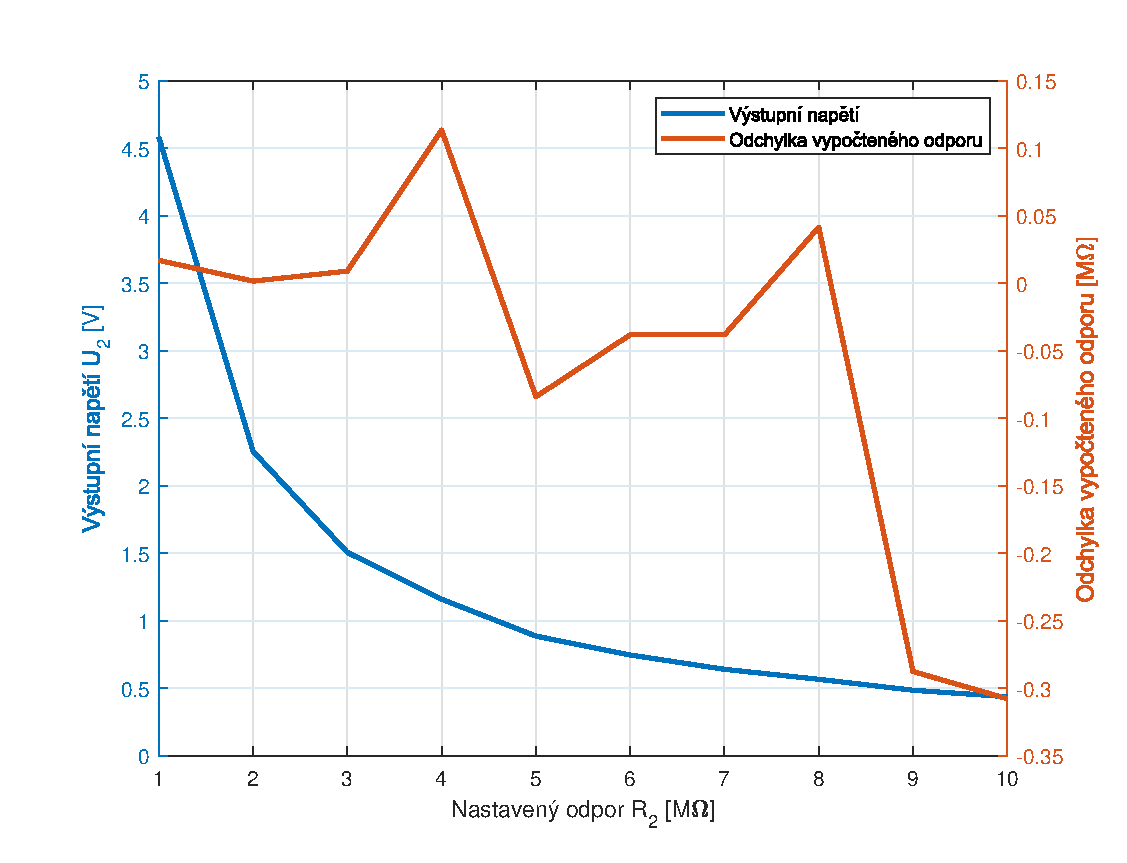
\includegraphics[width=0.9\textwidth]{mereni-r.eps}
    \caption{Chyba měření odporu synchronním detektorem}
    \label{mereni-r}
\end{figure}

\end{document}

